\documentclass[11pt]{article}

\usepackage[utf8]{inputenc} % Encoding
\usepackage{graphicx} % To include images
\usepackage{natbib} % For bibliography
\usepackage{amsmath} % For more complex equations
\usepackage{hyperref} % For hyperlinks

\usepackage{listings}



\title{CSCI2951O Project 1: Vehicle Customization}
\author{Name: Richard Tang, cslogin: rtang26, screenname: ginakonda}
\date{\today}

\begin{document}

\maketitle

\section{Introduction}
In this project, I implemented a CDCL-based SAT solver in Rust. The SAT solver attempts the
following optimizations: 2-watched literals, 1st-UIP clause learning and non-chronological
backtracking, EVSIDS, Glucose-based clause deletion, Conflict clause minimization, and Luby-based
restarts.

\section{Implementation}

To save space, the actual algorithm is detailed in the appendix, as well as some discussion on
programming language choice (see \ref{app:algo} and \ref{app:pl}). Some general implementation
notes:
\begin{itemize}
    \item Variables are mapped from the file values to an internal solver number, then mapped back
        on solution emission; this is done to prevent issues about gaps in numbering (as in
        \href{https://edstem.org/us/courses/55070/discussion/4403836}{this Edstem post}).
    \item Literals are assigned as such: \texttt{lit = 2 * var + sign}. This allows all literals to
        exist from $[0, n_{2\text{vars}+1})$, which provides easy indexing into vectors.
    \item The algorithm does not implement pure literal elimination. From literature review (and
        this \href{https://cs.stackexchange.com/q/44924}{corresponding StackOverflow post}), none of
        the major SAT solvers (PicoSAT, MiniSat, Chaff, etc) implement PLE for performance reasons.
\end{itemize}

I attempted various optimizations to improve performance:
\begin{itemize}
    \item \textbf{CDCL}: Instead of standard DPLL, I attempted to implement CDCL, with conflict
        analysis and clause learning. In particular, I maintained an trail of assigned variables,
        and their assignment reasons (either decision or propagating clause); then, on conflicts, I
        inspected the trail to find the first UIP (as defined in \cite{iccad} and
        \cite{GaneshVardi}). Most papers I referenced, however, didn't actually explain how to find
        the actual UIP, instead abstractly describing implication graphs; it turns out it's just a
        backtrack through the trail (a la reverse-BFS) to find the ``dominator node'' at the
        conflict decision level. I referenced the algorithm presented in MiniSat \cite{Een}.
        \begin{itemize}
            \item This also included non-chronological backtracking, which just popped off the trail
                and un-assigned variables until a desired decision level.
        \end{itemize}
    \item \textbf{2-Watched Literals}: Most references described how boolean constraint propagation
        took up the majority of runtime (which I eventually verified using \texttt{flamegraph}s; see
        \ref{app:fg}), so I attempted watched literals to optimize this. \cite{GaneshVardi} provided
        a good initial introduction to the algorithm; I then tried to implement the PicoSAT
        version with their pointer optimizations \cite{Biere}, but this proved too difficult to
        understand (and Rust didn't provide many required bit-packing language features in C/C++),
        so I again referenced the MiniSat\cite{Een} implementation, which maintained an occurrence
        list of watching clauses for \textit{each literal}; by ensuring the watched clauses were
        always indices $0$ and $1$, it optimized for access.
    \item \textbf{Glucose-based clause deletion}: After implementing CDCL, I noticed my learnt
        clause database kept growing, which made BCP incredibly slow (after a minute,
        \texttt{C1597\_024} had 1597 constraints and over 200k learnt clauses). Thus, I searched for
        clause deletion policies, eventually settling on Glucose's \cite{Glucose} LBD policy (which
        recorded the number of unique decision levels in each learnt clause).
    \item \textbf{Conflict Clause Minimization}: Like clause deletion, I noticed that learnt clauses
        had a large size (averaging $\approx 25$ per clause); to reduce this, I implemented conflict
        clause minimization from a follow-up MiniSat paper \cite{CCM} using self-subsuming
        resolution (essentially, if learned literals were implied by other literals or decisions,
        they are redundant), shrinking learnt clauses to average $\approx 8$ per clause.
    \item \textbf{EVSIDS}: For branch decision heuristics, I decided to implement EVSIDS. I
        originally wanted to implement VSIDS, but it involved a significant amount of iteration (for
        each update!); moreover, the actual EVSIDS implementation turned out to be quite easier.
        For decision heuristics in general, I referenced Chaff \cite{Chaff}, MiniSat \cite{Een}, and
        this survey paper \cite{Biere15}. 
    \item \textbf{Luby-based restarts}: I finally implemented Luby restarts; I wanted to try more
        specified in this paper \cite{Luby}, as well as Glucose-based restarts \cite{Glucose}, but
        unfortunately did not have enough time.
\end{itemize}

\subsection{Performance}

CDCL and 2-watch literals alone, for me, were insufficient to pass all clauses in the allotted time.
Glucose-based clause deletion, combined with conflict clause minimization, increased performance by
up to 350\%, but was still not sufficient. EVSIDS (instead of random assignment) further improved
performance by around 300\%, finally allowing me to pass all clauses within the time limit. Tuning
parameters on clause deletion, sometimes randomizing branch decisions and polarity, etc. did not
provide a significant improvement.

I tried implementing Luby restarts to speed up cases in which search entered a poor branch. Because
this caused a lot of restarts on UNSAT instances, though, it ended up slowing down my program, so I
disabled it by default.

I tried using multiple solver instances with different parameters and randomized decisions to find
instances faster, but I guess my algorithm is too deterministic (or too easily falls into the same
local minima), as this provided no performance improvement.

Besides algorithmic optimizations, I tried to use Rust's
\href{https://doc.rust-lang.org/rustc/profile-guided-optimization.html}{profile-guided optimization}
(PGO) to optimize compilation based on production examples (I used C1065\_064.cnf, U50\_1065\_038.cnf,
and U50\_4450\_035.cnf); however, this caused a slowdown by around 50\%, so I disabled it.


\subsection{Bugs}

Given its perhaps surprisingly slow performance, it's likely that I have latent implementation
errors (which are \textit{hopefully} just performance, not correctness, issues). Here are some
(mostly correctness) bugs that I discovered when implementing:
\begin{itemize}
    \item Due to my literal representation, I often got confused with the actual literal values (it
        didn't help that I had a custom boolean representation, where \texttt{True == 0}...); many
        times I forgot to flip the polarity when assigning.
    \item I forgot to un-assign values on backtracking, sometimes causing their reason clauses to be
        incorrectly filled on conflict analysis.
    \item In conflict analysis, I originally assigned \textit{unseen} literals as asserting
        literals, causing un-related reasons to be visited.
    \item I often failed to maintain invariants within the watch lists; watched values were supposed
        to be index $0$ and $1$, but I inconsistently changed clauses, causing duplicated and
        overridden literals. I also forgot to delete watchers, slowing down propagation.
    \item In clause deletion, I forgot to calculate LBD, and then I sorted it in reverse, causing
        the most \textit{important} clauses to be deleted.
    \item In EVSIDS computation, my floating point representation often overflowed, causing values
        to hit \texttt{inf} or \texttt{NaN}. This rendered EVSIDS values useless.
    \item So many off by ones! In decision level, 1-UIP backtracking, 2-watch literals maintenance,
        etc.  Indexing sucks :(
\end{itemize}

\section{Conclusion}

I spent roughly 40 hours implementing, debugging, and optimizing this project. Getting a concussion
mid-way greatly slowed down progress and made understanding certain algorithms---looking at you,
1-UIP conflict analysis---exceedingly difficult, but it was super fun to implement, and I'd like to
keep optimizing in the future.

\pagebreak

\appendix

\section{Implementation notes}

\subsection{Main algorithm}\label{app:algo}
The SAT solver consists of one large loop implementing the DPLL (CDCL) algorithm. Unit clauses are
repeatedly propagated: 
\begin{itemize}
    \item If no conflicts detected and all variables are assigned, we return SAT; otherwise, we
        decide the next variable using some heuristic, assign that variable, and re-propagate.
    \item If a conflict is detected, analyze the cause for the conflict, backtrack to the first
        UIP's decision level, and add that learned clause to the clause database. If the clause
        database is too large, clean it according to some policy. Re-propagate
\end{itemize}
If too many conflicts occur, there is an option to restart the search.

The algorithm was implemented following mostly Serdar's lecture notes, the paper ``On the
Unreasonable Effectiveness of SAT Solvers'' \cite{GaneshVardi}, the original Princeton Chaff paper
\cite{Chaff}, and the MiniSat paper \cite{Een}.

\subsection{Programming language choice}\label{app:pl}

I implemented the SAT solver in Rust. I was originally going to implement in C++, but I chose Rust
for a few reasons:

\begin{enumerate}
    \item Rust provides a rich ecosystem of both standard library and external ``crates'', with
        all sorts of functionality from custom hash functions to loggers to arena allocators. While
        C++ has a similar ecosystem, integrating it with a build system portably and linking during
        compilation proved to be a huge headache.
    \item In general, it's been too long since I've set up a CMake/C++ project; moreover, due to the
        inherent memory unsafety of C++, influency would result in many potentially terminal bugs.
\end{enumerate}

In general, this was a positive choice for me; Rust's strict ownership system and borrow checker
caught many of my programming mistakes or invalid memory accesses. As a result, on compilation, I
didn't encounter any(!) segfaults or undefined behavior from invalid variable modification (this is
not to say I didn't have bugs, only that they were all actual algorithm implementation bugs).

However, Rust's borrow checker did pose a nuisance in some cases. In particular, my
\texttt{CDCLSolver} object had many unrelated fields to store information (e.g. literal occurrence
lists, variable activity, etc.), to which simultaneous access should pose no problem; however,
because Rust's borrow checker forbids holding multiple mutable references at once, the compiler did
not allow this to compile. I experimented with
\href{https://doc.rust-lang.org/book/ch15-05-interior-mutability.html}{\texttt{RefCell}s and
interior mutability}, but due to its complexity (and associated runtime cost), I chose not to use
them. In the end, I ended up making copies of certain values then re-assigning them if I did need
multiple mutable accesses.

Patterns like this might suggest that Rust is still less performant than C/C++ in extreme cases,
where the borrow checker forbids correct optimizations.
\begin{itemize}
    \item Regardless, I think the developer experience of Rust far exceeds anything offered by
        C/C++.
\end{itemize}

\section{Flamegraphs}\label{app:fg}

I used flamegraphs to find bottlenecks within my code; as expected, much of the time was spent in
BCP. I didn't have time to completely re-factor my code or try different optimizations, but in the
future I'd like to attempt.

\begin{figure}[htpb]
    \centering
    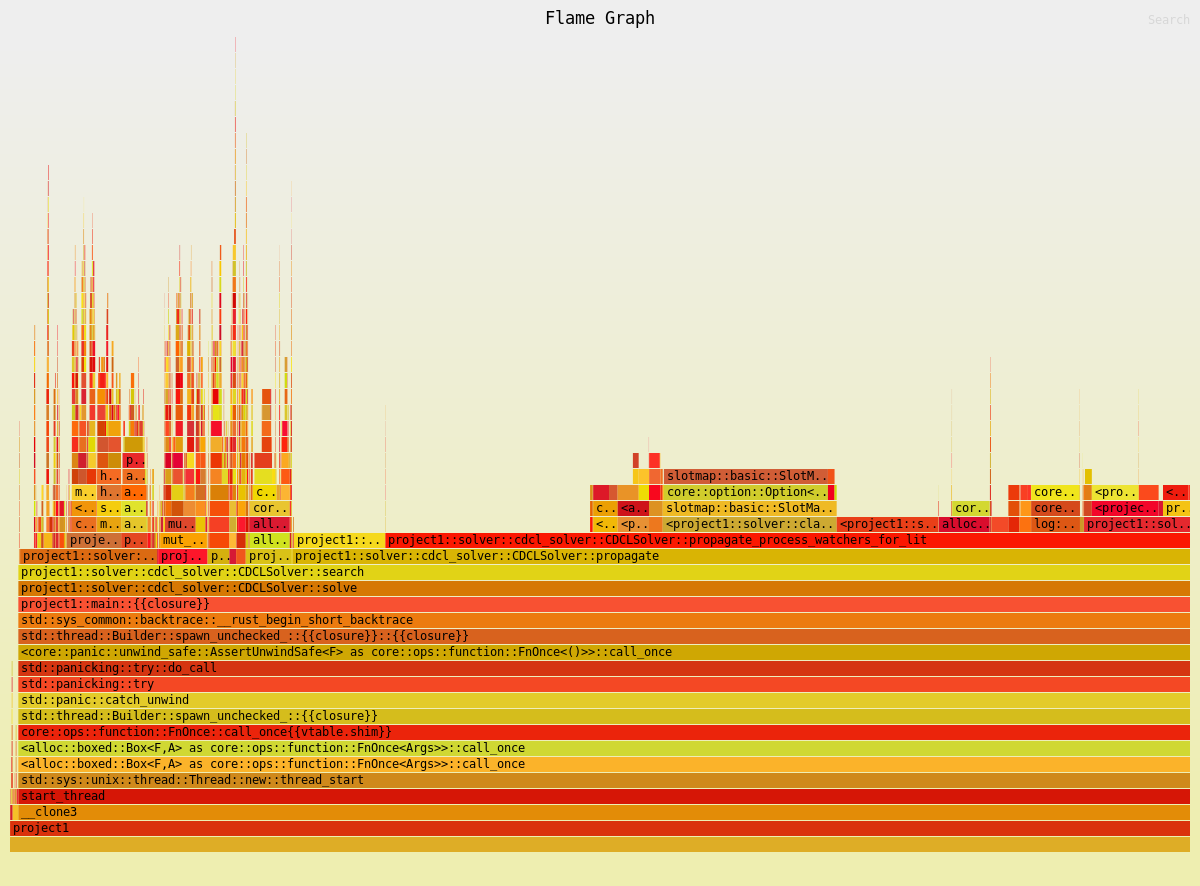
\includegraphics[width=0.75\textwidth]{U50_4450_035.png}
    \caption{Flamegraph for U50\_4450\_035.cnf. Note how \texttt{CDCLSolver::propagate} occupies
    almost 80\% of the execution time.}
    \label{fig:fg}
\end{figure}

\pagebreak

\bibliographystyle{plain}
\bibliography{references}

\end{document}

